\documentclass[11pt]{article} % use larger type; default would be 10pt
\usepackage[utf8]{inputenc} % set input encoding (not needed with XeLaTeX)

%%% BEGIN Article customizations

%%% PAGE LAYOUT
\usepackage{geometry} % to change the page dimensions
\geometry{a4paper} % or letterpaper (US) or a5paper or....
% \geometry{margin=1in} % for example, change the margins to 2 inches all round
\usepackage[parfill]{parskip} % Activate to begin paragraphs with an empty line rather than an indent

%%% FIGURES
\usepackage{graphicx} % support the \includegraphics command and options
\graphicspath{{../FIGURES/FIGURE_PDFS/}}

%%% PACKAGES
\usepackage{booktabs} % for much better looking tables
\usepackage{array} % for better arrays (eg matrices) in maths
\usepackage{paralist} % very flexible & customisable lists (eg. enumerate/itemize, etc.)
\usepackage{verbatim} % adds environment for commenting out blocks of text & for better verbatim
\usepackage{subfig} % make it possible to include more than one captioned figure/table in a single float
% These packages are all incorporated in the memoir class to one degree or another...

%%% HEADERS & FOOTERS
\usepackage{fancyhdr} % This should be set AFTER setting up the page geometry
\pagestyle{fancy} % options: empty , plain , fancy
\renewcommand{\headrulewidth}{0pt} % customise the layout...
\lhead{}\chead{}\rhead{}
\lfoot{}\cfoot{\thepage}\rfoot{}

%%% SECTION TITLE APPEARANCE
\usepackage{sectsty}
\allsectionsfont{\sffamily\mdseries\upshape} % (See the fntguide.pdf for font help)
% (This matches ConTeXt defaults)

%%% ToC (table of contents) APPEARANCE
\usepackage[nottoc,notlof,notlot]{tocbibind} % Put the bibliography in the ToC
\usepackage[titles,subfigure]{tocloft} % Alter the style of the Table of Contents
\renewcommand{\cftsecfont}{\rmfamily\mdseries\upshape}
\renewcommand{\cftsecpagefont}{\rmfamily\mdseries\upshape} % No bold!

%%% END Article customizations

%%% The "real" document content comes below...

\title{Reproducibility of SNP calling in multiple sequencing runs from single tumors}
\author{Dakota Z. Derryberry, Claus O. Wilke, Matthew C. Cowperthwaite}

\begin{document}
\maketitle

\section{Abstract}

A) What system are you studying?
B) Why is it important?
C) What is your research approach?
D) (optional) How is your research different from previous work?
E) What are the results of your research?
F) What conclusions can we draw from these results?

\section{Introduction}

A) What is the general field of study?
B) What is the specific question of the research?
C) Why is (a) and/or (b) important?
D) What has previously been done in this area?
E) How does your research differ?
F) (end with) a summary of the research described in this paper

Glioblastoma multiforme (GBM) is the most common and deadly primary brain tumor, with a median survival of 13.9 months and a 5-year survival of ~5\% \cite{TCGA-GBM-13}. Prognosis for patients with this disease remains poor despite significant research investment, due to the difficulty of surgical resection and the limited number of effective chemoteraputics. Like all cancers, GBM is an evolutionary disease caused by mutations and other alterations to normal glial cell lines. However, following substantial research efforts dedicated to identifying all of the mutations in an individual patient's tumor to try and identify causal variants, few precise causal elationships have been identified. There are two theories behind this descrepancy: First is the view that "GBM growth is driven by a signaling network with functional redundancy that permits adaptation" \cite{TCGA-GBM-13}. Second is the notion that batch effects and sequencing protocols, and thus the data on which genomic analyses are based, is imperfect. In reality, both of these views are probably correct. In this paper, we use data from doubly-sequnced GBM patients to investigate key attributes of the data and some of the most common computational processing pipelines.

 The largest effort behind this research is that of The Cancer Genome Atlas' Research Network, who first sequenced 206 GBMs in 2008 \cite{TCGA-GBM}. In the intervening years, this data set has grown to contain over 500 tumors with multiple types of molecular data, all made publicly available \cite{TCGA-GBM-13}. Each sample in the database contains data from a single patient's tumor and blood samples, allowing researchers to directly compare the two, and then compare sets of differences between tumor and "normal" tissue between patients.  While most of the ~600 sequencing samples in teh TCGA are from different patients, some 63 patients appear in the database twice, 55 having been seuqenced once each with two different DNA preparation methods, and 13 having been sequenced at two different times. In this paper,

Since it's publication in 2008, TCGA data has been used by researchers to investigate a variety of phenomena in GBM. (subtyping, drivres, pathways, targets) These successes aside, other results have caused some researchers to question what exactly is measured by the TCGA sequencing data. (the apper that showed all four subtypes in one tumor) (the more recent over time paper) (maybe another about heterogeneity) Sample preparation and sequencing methods, as well as computational analytical methods, indubitably influence sequencing results. In this paper, we begin to ask how.

WGS and WGA are different... We have 55 samples of each... Expectation is X, and we find as follows...

Same thing for the 13 samples...

Everyone must filter, (describe why)... We begin with the one SNP-caller SomaticSniper, and compare the filtered to the unfiltered date... We find as follows...

\section{Results}

\subsection{Unfiltered data: WGA v. WGS}

For 55 samples, TCGA has two identical data sets except for the sample preparation: one is whole genome sequencing (WGS) and the other is whole genome amplified sequencing (WGA). We calculated the number of mutations in each of these 110 samples (2 each from 55 patients). The number of mutations per sample ranged considerably, from XX to XX in the WGS samples and from XX to XX in the WGA samples. That the range is higher among the WGA samples is expected, because the amplification process may introduces mutations thereby artificially inflating the number of mutations in the dataset. To test this, we plotted the number of putative SNPs in the WGS and WGA sample preparation for each individual patient. As expected, for most patients, there were more mutations in the WGA sample than in the WGS sample (Figure 1). Surprisingly, not all exceptions had night numbers of mutations. One WGA sample with fewer than 50 mutaions had nearly 500 in the corresponding WGS sample; and one WGS sample with more than 200 mutations had only 200 in the corresponding WGA sample.

We next looked at the overlap between the called putative SNPs in the WGS and WGA samples. Although amplification may introduce new mutations, the mutations found in the WGS sample for each patient should be (mostly) a subset of those found in the WGA sample for that same patient. Although WGS may itself introduce some new mutations, the percent of WGS mutations that overlap with those found in the WGA sample should be significantly higher than the percent of WGA mutations found in the overlap with WGS. To test this, we calculated the overlap between the WGS and WGA samples for each patient. As expected, WGS samples have fewer non-overlapping putative SNPs than WGA samples (Figure 2). 

As seen in figure one, most WGS samples have around 500 putative mutaitons, and most WGA samples have around 1000, but there are a number of exceptions. We hypothesized that these samples, some containing as many as 10,000 mutations, were mostly corrupted data. To test this, we plotted the percentage of the WGA samples that overlaped with the corresponding WGS samples (as a measure of sample quality) against the total number of putative SNPs in the WGS sample (Figure 3). We expected a negative correlation, which would indicate that as the quality of the sample worsened, the number of mutations increased. Instead, we got a completely random distribution. This could indicate... (still trying to decide what I think this indicates)

\subsection{Unfiltered data: Time points}

\subsection{Filtering}

\section{Methods}

\subsection{Data and back-end processing}

All sequence data came from The Cancer Genome Atlas (TCGA) Research Network's Gliobastoma multiforme (GBM) data set \cite{TCGA-GBM}. We downloaded raw reads in .bam files from 68 patients using CGHub \cite{CGHub}. For each patient, data consisted of one set of reads taken from blood DNA, and two sets of reads taken from tumor DNA. In 55 cases, the two sets of reads from tumor DNA were one set of reads from whole genome sequencing (WGS) and one set of reads from whole genome sequencing with amplification (WGA). In 13 cases, the two sets of reads from tumor DNA were one set of reads pre-readiation treatment and one set post-radiation treatment. We developed a pipeline to align all reads to HG19. This pipeline used picard \cite{picard}, BWA \cite{BWA} for alignment, SamTools \cite{SAMtools}, GATK \cite{GATK}, and custom python code. We used SomaticSniper \cite{SomaticSniper} to align each tumor sequence with it's corresponding blood sequence, then filtered the SomaticSniper data using 6 custom filters. These removed putative SNPs (i) with a SomaticScore less than 40, (ii) within 10 bp from a high-quality indel, (iii) within 10 bp of another putative SNP, (iv) with a variant allele quality less than 20, (v) with a dbSNP \cite{dbSNP} identifier and fewer than 10x coverage, and (vi) that were loss of heterozygosity. All custom code is available in a github repository, and is available upon request.

\subsection{Analysis}

We used custom python scripts, available in the above github repository, to perform simple calculations and data operations. We used R \cite{Rsoftware} to do statistics and generate figures, and this code is also stored in a github repository and available upon request.  

\section{Discussion}

A) Start with a brief (one paragraph or less) summary fo your research, what you did and what you found
B) Put your results into perspective, discussing (i) what they imply and (ii) how they compare to existing literature
C) Address potential shortcomings. What could have gone wrong, which parts of the research might be misleading, are there any other caveats?
D) (optional) Describe implications for future research; are there obvious extensions?
E) (optional) End with a paragraph that again summarizes your research and highlights the most important findings

\section{Figures}

\begin{figure}
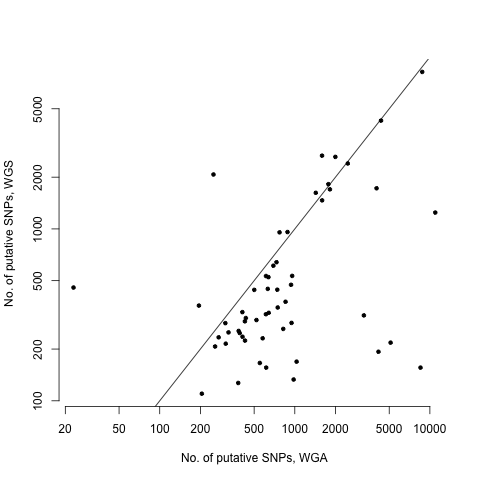
\includegraphics[scale=1.0]{C282_v_C484.png}
\caption{This figure plots the number of putative SNPs called by SomaticSniper (unfiltered) using the WGS v. WGA. Each point is a patient. The line is y=x, so points falling below the line agree with the hypothesis that whole genome amplification makes more mutations in a sample.}
\end{figure}

\begin{figure}
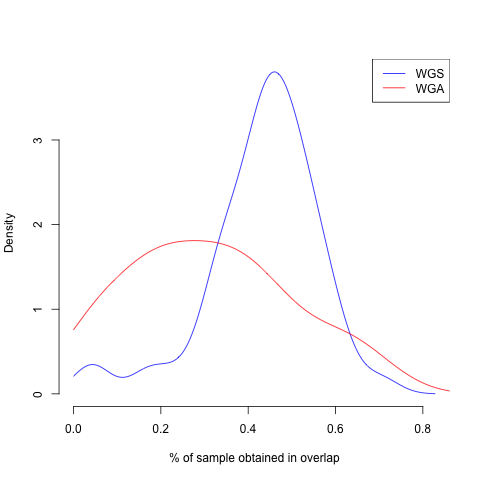
\includegraphics[scale=1.0]{unfiltered_overlap_WGS_WGA_together_densities.png}
\caption{This figure shows the density of the percentage of each WGS (blue) and WGA (red) sample that overlaps with the other sample from the same patient. The WGS distribution is higher and narrower, showing that the WGS samples overall have a higher percentage overlap than the WGA samples, and less range in this parameter. }
\end{figure}

\begin{figure}
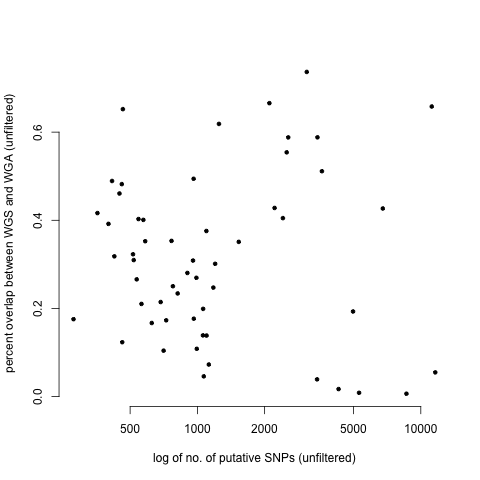
\includegraphics[scale=1.0]{unfiltered_total_muts_v_percent_overlap.png}
\caption{Plot of the percentage of the WGA samples that overlaped with the corresponding WGS samples (as a measure of sample quality) against the total number of putative SNPs in the WGS sample}
\end{figure}

\begin{figure}
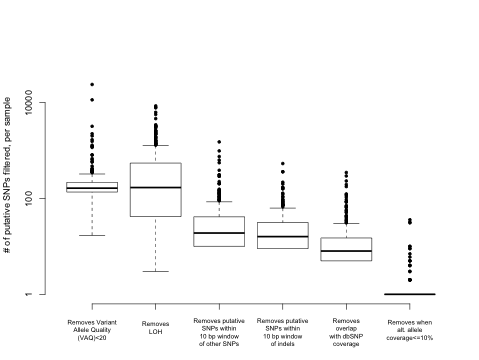
\includegraphics[scale=1.0]{boxplot_number_filtered.png}
\caption{Boxplot of the total number of putative SNPs removed by each of six filters, in each of 379 sequencing samples, from 311 patients. The x-axis gives the name of those filters that removed putative SNPs, and the y-axis gives, on a log scale, the number of mutations removed by a given sample.}
\end{figure}

\begin{figure}
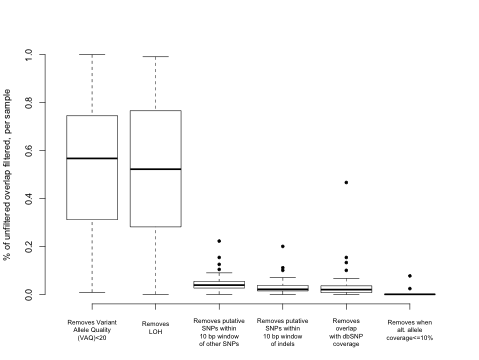
\includegraphics[scale=1.0]{boxplot_percent_overlap_filtered.png}
\caption{Boxplot of the percentage of putative SNPs making up the overlap between the WGS and WGA sequences of a single sample that was removed by a given filter. The x-axis describes the filters, and the y-axis gives the percentage of the overlap removed.}
\end{figure}

\bibliography{TCGA_bib}
\bibliographystyle{plain}

\end{document}

